\documentclass[letterpaper,11pt]{article}

%packages
\usepackage{amsfonts}
\usepackage{graphicx}
\usepackage[left=2cm,top=2cm,right=2cm,bottom=1.5cm,head=.5cm,foot=.5cm]{geometry}
\usepackage{url}
\usepackage{multirow}
\usepackage{longtable}
\usepackage{subfig}
\usepackage{float}
\usepackage{setspace}
\usepackage{lineno}
\usepackage{natbib}
\usepackage{amsmath}
\usepackage{authblk}
\usepackage{xr}
\usepackage{relsize}
\usepackage{tikz}
\usepackage{Sweave}

%external documents
\externaldocument[SI-]{SupMat}

%new commands and so on
\providecommand{\keywords}[1]
{
  \small	
  \textbf{\textit{Keywords---}} #1
}

\DeclareMathOperator{\E}{\mathbb{E}}% expected value
\DeclareMathOperator{\var}{var}
\DeclareMathOperator{\cov}{cov}
\DeclareMathOperator{\cor}{cor}
\DeclareMathOperator{\mean}{mean}
\DeclareMathOperator{\se}{se}
\DeclareMathOperator{\sd}{sd}
\DeclareMathOperator{\prob}{P}

%attempt 1 at nat and sharp
%\newcommand{\nat}{\mathlarger{\natural}}
%\newcommand{\shp}{\mathlarger{\sharp}}

%attempt 2 at nat and sharp
%\newcommand{\nat}{\raisebox{1pt}{\mathsmaller{\mathsmaller{/\hspace{-2pt}/}}}}
%\newcommand{\shp}{\#}

%attempt 3 at nat and sharp
\newcommand{\nat}{%
\text{\hspace{-1.5pt}
\begin{tikzpicture}[scale=1.8]%
\draw (.333ex,0) -- (.333ex,1ex);%
\draw (.666ex,0) -- (.666ex,1ex);
\end{tikzpicture}%
}}
\newcommand{\shp}{%
\text{\hspace{-1.5pt}
\begin{tikzpicture}[scale=1.8]%
\draw (0,.333ex) -- (1ex,.333ex);%
\draw (0,.666ex) -- (1ex,.666ex);%
\draw (.333ex,0) -- (.333ex,1ex);%
\draw (.666ex,0) -- (.666ex,1ex);
\end{tikzpicture}%
}}
\newcommand{\test}{%
\text{
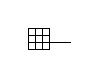
\begin{tikzpicture}[scale=1.8]%
\draw (0,0) -- (1ex,0ex);
\draw (0,0) -- (0ex,1ex);
\draw (0,1ex) -- (1ex,1ex);
\draw (1ex,0) -- (1ex,1ex);
\draw (0,.333ex) -- (2ex,.333ex);%
\draw (0,.666ex) -- (1ex,.666ex);%
\draw (.333ex,0) -- (.333ex,1ex);%
\draw (.666ex,0) -- (.666ex,1ex);
\end{tikzpicture}%
}}

\newcommand{\olr}{\overline{r}}
\newcommand{\olrs}{\overline{r}^{\shp}}
\newcommand{\olrn}{\overline{r}^{\nat}}
\newcommand{\bs}{\backslash}

%header material for paper
\title{Working document to try to explain why/how ATAs influence coexistence in an intuitive way for referee 3}
\date{}

\author[a,b]{Pimsupa Jasmin Albert}
\author[a,c,*]{Daniel C. Reuman}

\affil[a]{Department of Ecology and Evolutionary Biology and Center for Ecological Research, University of Kansas}
\affil[b]{Environmental Studies Program and Department of Biology, University of Oregon}
\affil[c]{Laboratory of Populations, Rockefeller University}
\affil[*]{Corresponding author, reuman@ku.edu}

%for dealing with line numbers bugs having to do with equations
\let\oldequation\equation
\let\oldendequation\endequation
\renewenvironment{equation}
  {\linenomathNonumbers\oldequation}
  {\oldendequation\endlinenomath}
\let\oldalign\align
\let\oldendalign\endalign
\renewenvironment{align}
  {\linenomathNonumbers\oldalign}
  {\oldendalign\endlinenomath}

\begin{document}

\maketitle

\section{Initial thinking}

This approach is nothing analogous to attempts I have seen to intuitively explain storage effects. Part of the
reason for that is that those attempts may be rooted at least partly in the Chesson theory, which assumes
small noise. We no longer make that assumption, and we already know (or strongly suspect, based on the 
intuition provided by Steve Ellner) that ATAs will not make any difference under a small noise assumption,
because under such an assumption the approximations of Chesson are good. The approach described here also has other differences, 
discussed below. One major shortcoming is that this approach provides little ecological intuition as to what ATA
effects precisely are, even if it does (I hope) make it seem not only plausible but expected that they should
frequently matter. And it provides some mathematical intuition that could prehaps be substituted for purely
ecological intuition in some sense. I look forward to discussing this approach with Jasmin before possibly putting some version 
of it in the paper.

We mainly consider the lottery model. Though we begin with some more general notation, we quickly make an
assumption that I think will only hold for the lottery model.
We assume, as usual, that for whatever model we consider (a 2-species model), we can write $r_i$ as
a function of $E_i$ and $C_i$, and $r_i$ is an increasing function of $E_i$ and decreasing function
of $C_i$. Then ATA effects are defined as
\begin{align}
\Delta_i^{[EC]} &= (\olr_{i \bs i} - \olr_{j \bs i})-(\olrn_{i \bs i} - \olrn_{j \bs i}) \label{eq:ATAeffects1}\\
&= (\olr_{i \bs i} - \olrn_{i \bs i}) - (\olr_{j \bs i} - \olrn_{j \bs i}) \label{eq:ATAeffects2}\\
&= (\olr_{i \bs i} - \olrn_{i \bs i}).
\end{align}
The third term in (\ref{eq:ATAeffects2}) is $0$ because that represents growth of $j$ in a steady-state scenario,
and the fourth term is $0$, for the lottery model, because of reasoning in S5.1. So here is where we are 
getting specific to the lottery model, as warned above. Maybe the next iteration of this thinking should 
consider what happens when that fourth term does not vanish. Can we generalize? I think we can - see below for
some efforts to generalize which were added later.

For the lottery model, we have 
\begin{align}
\Delta_i^{[EC]} &= (\olr_{i \bs i} - \olrn_{i \bs i}) \\
&= \E \left[ \ln \left( 1-\delta+\frac{E_i}{C_{i \bs i}} \right) \right] - \E \left[ \ln \left( 1-\delta+\frac{E_i^\nat}{C_{i \bs i}^\nat} \right) \right]. \label{eq:DeltaTerm1} 
\end{align}
The first term of (\ref{eq:DeltaTerm1}) is the average of the function $\ln(1-\delta+x/y)$ over the bivariate 
distribution $(E_i,C_{i \bs i})$, whereas the second term of that expression is the average of the same
function over the distribution $(E_i^\nat,C_{i \bs i}^\nat)$. We can visualize these averages pretty easily and 
effectively (see below) for specific distributions, and it helps to see how ATAs can influence coexistence.
Fig. \ref{thefig} shows this visualization. For the log-normal fecundities model (A-D), the average value of the 
function over the green points should be about the same on each panel as over the black points, 
corresponding to the fact that $\Delta_i^{[EC]}$ is close to zero for the parameters used (see Fig. 2). 
On the other hand, for the beta-fecundities model for left-tail associated noise (E, F), the average of the function 
over the black points is obviously going to be bigger than its average over the green points, corresponding to the 
fact that, for these parameters, $\Delta_i^{[EC]}$ is negative (Fig. 3).
For the beta-fecundities model for right-tail associated noise (G, H), the average of the function 
over the black points is obviously going to be smaller than its average over the green points, corresponding to the 
fact that, for these parameters, $\Delta_i^{[EC]}$ is positive (Fig. 3).

\begin{figure}
\includegraphics[width=\textwidth]{../results_figs/PostHocExplanatoryFig.jpg}
\caption{Pictorial representation of $\E \left[ \ln \left( 1-\delta+\frac{E_i}{C_{i \bs i}} \right) \right]$ and 
$\E \left[ \ln \left( 1-\delta+\frac{E_i^{||}}{C_{i \bs i}^{||}} \right) \right]$ for the 
log-normal-fecundities lottery model (A-D) and the beta-fecundities lottery model (E-H),
for left-tail associated noise (A, B, E, F), and for right-tail associated noise (C, D, G, H).
The color and contours show $\ln(1-\delta+x/y)$, whereas the green points on each panel show a sample from
the distribution $(E_i,C_{i \bs i})$ and the black points show a sample from the distribution 
$(E_i^{||},C_{i \bs i}^{||})$. Thus the average value of the function over the green points minus its
average value over the black points is a good approximation of $\Delta_i^{[EC]}$. Here $i=1$ and
$j=2$. We used parameters $\sigma=1$, $\mu_1 = 0$, and $\mu_2 = 0.5$ for the log-normal fecundities
model; $\eta_1 = 1$ and $\eta_2 = 1.2$ for the beta-fecundities model; and $\delta=0.6$
for both models. Results are plotted on both linear (A, C, E, G) and log (B, D, F, H) 
scales for readability.}\label{thefig}
\end{figure}

Viewing $\Delta_i^{[EC]}$ as an average of a function over a set of points distributed in a certain way
(with ATAs) minus an average of the same function over a set of points distributed in another way
(with ATAs removed) makes it clear why we would expect to commonly see substantial ATA effects 
on coexistence: removing ATAs really changes the way points in a bivairate distribution are 
distributed, in a way that can interact strongly with averaging over a function representing growth of
a potential invader. In fact, it seems clear that only very special functions will give the exact same results 
when averaged over a typical distribution with ATAs or with ATAs removed.

Growth from rarity, $\olr_{i \bs i}$ is an average of the individual growth rates which pertain across
years, and those values depend on the details of the distribution of $E$ and $C$. If we use 
$E_i$ and $C_{i \bs i}$, well then of course we will tend to get different values
from if we use $E_i^\nat$ and $C_{i \bs i}^\nat$. The question is just how much different, which is what 
we have sought to answer with this paper for lottery model and experimental examples. 

\section{Efforts to generalize}

Equation (\ref{eq:ATAeffects2}) is what we had prior to specifying to the lottery model. 
Above, we've considered the first two terms, which are the average of $r_i(E_i,C_i)$ over 
the distribution $(E_i,C_{i \bs i})$ minus the average of the same function
over $(E_i^\nat,C_{i \bs i}^\nat)$. But the last two terms of (\ref{eq:ATAeffects2})
are the average of $r_i(E_j,C_j)$ over the distribution $(E_j,C_{j \bs i})$ minus the 
average of the same function over $(E_j^\nat,C_{j \bs i}^\nat)$. So the same basic
ideas apply here as in the lottery model case, it's just that we have to make two comparisons 
of growth functions averaged over distributions, one comparison for the invader, $i$,
and the other for the resident, $j$. Again, essentially any model will have 
non-zero value of (\ref{eq:ATAeffects2}) -- only models designed as counterexamples
should typically have a precisely zero value for that expression. So ATAs will always
matter to some extent for coexistence. It's just a question of how much, for real systems. 
And, as far as can tell, that can only be answered by computing these quantities for
several real systems. We've shown that, at least for some systems, the quantities 
can be meaningfully large.

\section{Additional commentary/thinking by writing}

OK, it seems clear to me that basically any meanigful change to the distribution 
$(E,C)$ will typically alter the average value of the nonlinear function $r(E,C)$ 
over that distribution. There are many ways to decompose the growth rate 
$\olr_{i \bs i}$ through a series of alterations of the distribution $(E,C)$. 
Ellner et al. also make this point in their 2019 paper. The original Chesson 
theory is probably the most natural decomposition under a weak noise assumption,
but Ellner et al. and our paper make it clear there are other ways that may make
more sense, in some circumstances, if noise is not weak. 

\section{Ecological explanation}
\subsection{Basic MCT}
Under Modern Coexistence Theory, the outcome of coexistence is determined by 
niche differences and fitness differences (Chesson 2000, Adler 2007). 
When niche differences overcome fitness differences, coexistence is possible. 
Niche differences are driven by stabalizing mechanisms (such as the storage effect), 
which are defined as mechanisms that cause a species to limit itself more than it 
limits others, i.e., the species experiences more intraspecific competition than 
interspecific competition. 

\subsection{Storage effect and how ATAs can change it}
The storage effect stably contributes to coexistence through 
temporal niche partitioning with EC covariance and buffered population growth.
Under invader-resident analysis [rare-common], EC covariance limits the resident by 
coupling high environmental responses with high intraspecific competition. The magnitude
of the storage effects then depends on the EC covariance of the invader. Because the 
invader is introduced into the resident steady state community at close to zero density, 
its C is only a result of interspecific competition from the resident. Thus, the more closely 
related the invader's EC relationship is, the more interspecific competition it experiences, 
destabalizing coexistence. Equivalently, invader EC relationships with more spread stably
contribute to coexistence (through the storage effect). As seen in Fig. \ref{thefig}, ATAs in 
the invader EC relationship changes its bivariate distribution to both have more spread 
about the "central line" and be more densely situated about the "central line".  
%is central line like niche overlap line? species association line?  
When the invader's EC relationship has more spread (more density in values far away from 
the central line) than what the invader's EC relationship would be if it was symmetric, 
the ATA effect is positive. More specifically, points to the right of the central line are where environmental response is high and competition is low. When points fall in this plane, is when species can "store" the beneficial effects of a good environment to counteract when conditions are less ideal. Thus when the EC relationship is less spread, the invader is less able to recover from rare because the points are far away from the beneficial extremes. 
I think this related to the subadditivity criteria of storage effect, i.e., buffered population growth which is related to nonlinear averaging. Subaddivity/ buffered popualtion growth is when species growth rate responses to competition are less affected/sensitive to bad environmental conditions and more affected and sensitive when conditions are good. So it is nonlinear. So points in the beneficial extremes are when the invader can take advantage of the nonlinear averaging that comes with buffered population growth. ATA'd EC relationships have different distribution of points compared to one that is symmetric with the same marginals and correlation so the asymmetry changes whether or not points are in the beneficial extremes.   

\subsection{How can ATAs in the EC relationship arise?}
\emph{Water limitation.} Everyone depends on water. When water is limited niches become less different. So the invader's EC relationship in low values of environmental response is more correlated to the competitive pressure it experiences from the resident since the resident is also experiencing water limitation and will be in its low environmental response values. When water is not the limiting factor, environmental responses take on higher values and thus, the EC relationship may be more spread. 

\emph{Pollinator competition}. When environmental conditions are bad, specialized pollinators are less abundant. Two plant species may have to depend more on the generalist species, thus niches become less different.  (Niche overlap in bad environment leading to left tailed ATA)

\subsection{Dan thoughts 2023 07 26 - planned for inclusion in the Discussion}

% %Attempt 1 - not as good, Dan thinks. May be slightly misleading. See below for attempt 2.
% %
% %I have in mind that the following paragraph will go i the Discussion, with maybe a sentence
% %or two in the Intro as a preview of coming attractions.
% Just as for storage effects, temporal niche differentiation is necessary in order for ATA
% effects to materialize. This makes intuitive sense because temporal niche differentiation is 
% also a prerequistite of storage effects [\cite{Chesson_1994} and Box 2 of \cite{StumpVasseur2023}],
% and ATA effects are a part of storage effects, but see
% SI section X for a detailed explanation. 
% %Topic sentence follows. Possibly we can state something like this in the Intro and say
% %we explain it in the Discussion after formalizing the extent to which ATAs are important.
% If temporal niche differentiation occurs, ATA effects essentially capture the influence of asymmetries 
% in the extent to which storage effects can occur in environmentally good versus bad years,
% as we here explain.
% %
% These asymmetries can make a big difference to total storage effects and coexistence,
% as some of our analyses showed.
% %
% If temporal niche differentiation occurs
% but is partial (as will be typical), the quantities $E$ and $C$ experienced by a currently scarce 
% species (i.e., $E_i$ and $C_{i \bs i})$ will be positively but imperfectly correlated. 
% %
% Storage effects can occur if some buffering mechanism reduces losses in bad years so that
% gains in good years can more than make up for them. 
% %
% Bad years happen whenever the negative effects of $C$ outweigh any 
% positive effects of $E$; but this can occur
% both when 1) $E$ is moderately favorable but $C$ is very strong, as well as when 2) $E$ is very unfavorable,
% or moderately unfavorable and $C$ is not too weak.
% Conversely, good years happen whenever positive effects of $E$ outweigh negative effects of $C$;
% but this can occur when 1) $E$ is very favorable, or moderately favorable and $C$ is not too strong,
% as well as when 2) $E$ is moderately unfavorable but $C$ is very weak. 
% %
% ATA effects essentially quantify the asymmetry of storage that occurs when 
% $E$ and $C$ are both higher than average (the cases 1, above); versus storage that occurs 
% when $E$ and $C$ are
% both lower than average (the cases 2, above). 
% %
% The distinction is an important one because it corresponds to temporal niche differentiation
% which occurs under two very different sets of environmental conditions, possibly via
% different ecological or physiological mechanisms.
% %
% Details, applications, and examples of this intuition 
% are in SI section X, and these ideas are also used there to provide 
% intuitive explanations for the relative differences in the importance
% of ATA effects between our log-normal and beta fecundities lottery models.
% %DAN: You ought to also mention explaining differences with the diatom system,
% %if you figure out an explanation.

%Attempt 2 below - better than the above, but may need to be simplified a bit more,
%if possible
%
Just as for storage effects, temporal niche differentiation is necessary for ATA
effects. This makes intuitive sense because temporal niche differentiation is 
also a prerequistite of storage effects [\cite{Chesson_1994} and Box 2 of \cite{StumpVasseur2023}],
and ATA effects are a part of storage effects, but see
SI section X1 for a detailed explanation. 
%
Assuming that temporal niche differentiation is present, how do ATA effects then happen?
We here offer an intuitive explanation. 
%
If temporal niche differentiation occurs
but is partial, the $E$ and $C$ experienced by a currently scarce 
species (i.e., $E_i$ and $C_{i \bs i})$ will be positively but imperfectly associated, 
and the association may be asymmetric. 
%
Storage effects can occur if some buffering mechanism reduces losses in bad years so that
gains in good years can more than make up for them. 
%
Bad years happen when the negative effects of $C$ outweigh any 
positive effects of $E$; but this can occur
both 1) when $E$ is moderately favorable but $C$ is very strong, as well as 2) when $E$ is very unfavorable,
or moderately unfavorable and $C$ is not too weak.
Conversely, good years happen when positive effects of $E$ outweigh negative effects of $C$;
but this can occur 1) when $E$ is very favorable, or moderately favorable and $C$ is not too strong,
as well as 2) when $E$ is moderately unfavorable but $C$ is very weak. 
%
It turns out that the potential for storage to occur when 
$E$ and $C$ are both higher than average (the cases 1, above); versus the potential  
when $E$ and $C$ are
both lower than average (the cases 2) are not necessarily equivalent.
Depending on the growth rate function, $r(E,C)$, storage potential may differ
across the spectrum from 1 to 2.
%
ATA effects are the extent to which asymmetries of association between $E$ and 
$C$ are aligned with the potential for storage across the dichotomy 1 versus 2.
If $E$ and $C$ are strongly associated in the parts of their distribution where
storage potential is high, ATA effects will be relatively low, and vice versa.
A comparison is made to a benchmark of symmetric association between $E$ and $C$.
%
ATA effects therefore help quantify different degrees of temporal niche differentiation 
occuring under different sets of environmental conditions (such as cases 1 and 2), possibly via
different ecological or physiological mechanisms.
%
Details, applications, and examples of this intuition 
are in SI section X2, and these ideas are also used there to provide 
intuitive explanations for the relative differences in the importance
of ATA effects between our log-normal and beta fecundities lottery models.
%DAN: You ought to also mention explaining differences with the diatom system,
%if you figure out an explanation.

\subsection{SI section X1 corresponding to the thoughts above, call it Temporal niche differentiation is necessary for ATAs}\label{SIsect:temporal_niche_diff}

Just as for storage effects [see \cite{Chesson_1994} and Box 2 of \cite{StumpVasseur2023}], 
temporal niche differentiation is necessary in order for ATA
effects to materialize; we here explain why, in detail. ``Lack of temporal niche differentiation'' can be interpreted
to mean that species respond in identical ways to environmental fluctuations. 
In a two-species model such as those we consider, this should mean a monotonically
increasing relationship between $E_i$ and $C_{i \bs i}$. The former is the environment
as perceived by species $i$. The latter is competition that a scarce invader $i$ experiences
in a monoculture of $j$, and that competition comes only from $j$ (because $i$ itself
is scarce), so should correspond to the environmental response of $j$. If 
$E_i$ and $C_{i \bs i}$ are monotonically related, then $(E_i,C_{i \bs i})$
and $(E_i^\nat,C_{i \bs i}^\nat)$ are distributed in the same way, so 
$\E[r_i(E_i,c_{i \bs i})]-\E[r_i(E_i^\nat,c_{i \bs i}^\nat)]=0$.
Therefore, 
\begin{align}
\Delta_i^{[EC]} &= (\olr_{i \bs i}-\olr_{j \bs i})-(\olr_{i \bs i}^\nat - \olr_{j \bs i}^\nat) \\
&= \olr_{i \bs i}-(\olr_{i \bs i}^\nat - \olr_{j \bs i}^\nat) \\
&= \E[r_i(E_i,C_{i \bs i})]-\E[r_i(E_i^\nat,C_{i \bs i}^\nat)]+\E[r_j(E_j^\nat,C_{j \bs i}^\nat)] \label{eq:expri}\\
&= \E[r_j(E_j^\nat,C_{j \bs i}^\nat)].
\end{align}
But we already know $\E[r_j(E_j^\nat,C_{j \bs i}^\nat)]=0$
because there is no niche differentiation between $j$ and itself, so 
$E_j$ and $C_{j \bs i}$ should be monotonically related. So 
$\E[r_j(E_j^\nat,C_{j \bs i}^\nat)] = \E[r_j(E_j,C_{j \bs i})]=0$, giving
$\Delta_i^{[EC]}=0$. So temporal
niche differentiation, interpreted as Spearman correlation between 
$E$ and $C$ less than $1$, is necessary for ATA effects on coexistence to 
materialize.

\subsection{SI section X2 corresponding to the thoughts above, call it Intuition and 
examples for ATAs}\label{SIsect:intuition_examples}

If temporal niche differentiation occurs but is partial, 
then $E_i$ and $C_{i \bs i}$ will be positively but imperfectly correlated with
each other, corresponding to similar but non-identical responses of species to
environmental fluctuation (see SI section \ref{SIsect:temporal_niche_diff}); 
but how do ATA effects then happen? We here extend the intuition
introduced in the Discussion and provide examples. 

Storage can occur if population
increases during good years outweigh decreases during bad years. For instance,
if $r_i(E_i,C_{i \bs i})$ is very large when the balance of $E_i$ and 
$C_{i \bs i}$ is favorable, but only moderately small when this balance is
unfavorable, the expected value $\E[r_i(E_i,C_{i \bs i})]$ in (\ref{eq:expri})
will be positive. But the potential for such storage of population growth
may differ between when $E_i$ and $C_{i \bs i}$ are both high compared
to when they are both low. 
For instance, for the beta fecundities lottery model, $E_i/C_{i \bs i}$, a quantity
which features prominently in $r_i(E_i,C_{i \bs i})=\log(1-\delta+E_i/C_{i \bs i})$,
takes values bounded above by $\frac{2\eta_i \delta}{\eta_j}$ 
and bounded below by $\frac{\eta_i \delta}{2 \eta_j}$ when $E_i$ and $C_{i \bs i}$
are both in the upper halves of their assumed beta distribtions (recall that 
these quantities were assumed to be distributed, respectively, as $\eta_1 \beta$
and $\eta_2 \beta/\delta$ for $\beta$ a beta-distributed random variable with parameters 
$0.5$ and $0.5$). These bounds are separated only by a factor of four. 
On the other hand, when $E_i$ and $C_{i \bs i}$ are both in the lower halves 
of their distributions, $E_i/C_{i \bs i}$ can take any positive value because
then either $E_i$ or $C_{i \bs i}$ can take values arbitrarily close to $0$. 
Because values of $E_i/C_{i \bs i}$ have the potential to be much larger when 
$E_i$ and $C_{i \bs i}$ are both in the lower halves of their distributions
than when these quantities are both in their upper halves, and because
the growth rate, $\log(1-\delta+E_i/C_{i \bs i})$, buffers low values of 
$E_i/C_{i \bs i}$ (the infemum of the growth rate is $\log(1-\delta)$, whereas the supremum is
infinite), the storage effects contributed by the left tails of 
$E_i$ and $C_{i \bs i}$ have the potential to be much greater than those contributed
by the right tails. Essentially, values of $\log(1-\delta+E_i/C_{i \bs i})$
occurring when $E_i$ and $C_{i \bs i}$ are both in the upper halves of their
distributions can never exceed $\log(1-\delta+\frac{2\eta_i \delta}{\eta_j})$,
whereas values ocurring when $E_i$ and $C_{i \bs i}$ are both in the lower
halves of their distributions can be arbitrarily large (though with decreasing 
probability for larger values). Apparently, the years with the most potential to 
contribute to storage
effects for the beta-fecundities lottery model are those for which the environment
is actually poorer than average, because, for those years, competition can be very low,
so that the ratio $E/C$ is large. Years for which the
environment is exceptionally good actually cannot contribute much to storage effects for 
this model, because for those years, $E/C$ cannot be large.
It is the imbalance between $E$ and $C$ that allows for storage effects. 
Counterintuitively, for this model, that imbalance is greatest when the environment is 
poor. This result is counterintuitive because one may be used to thinking of storage effects
occuring when reproductive pulses from environmentally good years sustain the population
through environmentally poor years. But, in fact, good years for population growth may
happen principally when the environment is poor, if those are also the times when 
competition is very low, as for this model.

Fig. \ref{fig:beta_fecundidities_explanatory} provides quantitative backing to
the ideas of the prior paragraph. The growth function $\ln(1-\delta+E/C)$ that pertains 
to the lottery model
is plotted with colors and contours on Fig. \ref{fig:beta_fecundidities_explanatory}A-C.
Samples were taken from the distribution $(E_i,C_{i \bs i})$ for the beta 
fecundities lottery model for left- and right-tailed 
associations between $E_i$ and $C_{i \bs i}$, and are plotted as
points on Fig. \ref{fig:beta_fecundidities_explanatory}A and C, respectively. 
Samples were also taken from the distribution $(E_i^\nat,C_{i \bs i}^\nat)$
(which is the same regardless of whether the original $(E_i,C_{i \bs i})$
distribution showed left- or right-tail association) and are plotted on 
Fig. \ref{fig:beta_fecundidities_explanatory}B. 
The dashed lines labelled $L_2$ on A-C separate the upper-right $50\%$
of each distribution from the lower-left $50\%$. The dashed lines labeled
$L_1$ separate the upper-left $50\%$ from the lower-right $50\%$.
The quantity $\E \left[ \ln \left( 1-\delta+\frac{E_i}{C_{i \bs i}} \right) \right]$ can be
well approximated for left- and right-tail associations by averaging function 
values, depicted with color and contours, over the points on panels A and C, respectively. The quantity
$\E \left[ \ln \left( 1-\delta+\frac{E_i^{||}}{C_{i \bs i}^{||}} \right) \right]$
can be well approximated by averaging function 
values over the points on B. So ATA effects for the model with left-tail association
between $E_i$ and $C_{i \bs i}$ (respectively, right-tail association) are given by 
computing the average function value over points on panel A (respectively, C)
and then subtracting the average function value over points on panel B.
Contributions to the storage effect of points in the left portions of 
the $E,C$ distribution (the region labeled ``left'' on panels A and C)
can be accurately estimated by averaging function values across
points in that region; likewise storage contributions of points in the 
``right'' region can be estimated by averaging function values over 
points in that region. 

The details of the averaging process described above are pictured in 
Fig. \ref{fig:beta_fecundidities_explanatory}, panels D-F;
we now describe how. 
Signed distances of points on Fig. \ref{fig:beta_fecundidities_explanatory} 
A-C from the lines $L_1$ correspond to 
the quantities $\log_{10}(E_1/C_{1 \bs 1})$ on A, C and to 
$\log_{10}(E_1^\nat/C_{1 \bs 1}^\nat)$ on B. The distributions of these 
quantities across points to the left of $L_2$ are pictured 
in the lower horizontal-axis historgrams on panels D-F, respectively;
and distributions for points to the right of $L_2$ are 
pictured in the upper horizontal-axis histograms. 
For the left-tailed case (A, D), distributions to the  




\begin{figure}
\includegraphics[width=\textwidth]{../results_figs/PostHocExplanatoryFig_betaFecund.jpg}
\caption{A detailed look at ATA effects for the beta fecundities lottery model.
The figure gives a pictorial representation of the calculation of  
$\E \left[ \ln \left( 1-\delta+\frac{E_i}{C_{i \bs i}} \right) \right]$ (A, C, D, F) and 
$\E \left[ \ln \left( 1-\delta+\frac{E_i^{||}}{C_{i \bs i}^{||}} \right) \right]$ (B, E)
for the model, considering both left- (A, D) and right-tail (C, F) associations
between $E_i$ and $C_{i \bs i}$.
The colors and contours on A-C $\ln(1-\delta+E/C)$, whereas the points show a sample
from the distribution $(E_i,C_{i \bs i})$ (A, C) or $(E_i^{||},C_{i \bs i}^{||})$ (B).
The quantity $\E \left[ \ln \left( 1-\delta+\frac{E_i}{C_{i \bs i}} \right) \right]$ can be
well approximated for left- and right-tail associations by averaging function 
values over the points on panels A and C, respectively. The quantity
$\E \left[ \ln \left( 1-\delta+\frac{E_i^{||}}{C_{i \bs i}^{||}} \right) \right]$
can be well approximated by averaging function 
values over the points on B. Values of $\log_{10}(E/C)$ for the points on A-C correspond 
to signed distances of the points from the upward sloping dashed lines. 
We used parameters $\eta_1 = 1$, $\eta_2 = 1.2$, and and $\delta=0.6$. }\label{fig:beta_fecundidities_explanatory}
\end{figure}


\bibliographystyle{ecology_letters2}
\bibliography{refs}

\end{document}